\subsection{The picture environment}

This is the most interesting capability of \LaTeX\ although it might be
considered as 'fiddly' by some users, as it requires some trial and error, but
it can be very useful in some cases (eg. Having a lot of figures with chemical
structures and getting them cross-referenced and numbered correctly).

The example in the figure \ref{fig:plot2} just shows how one could do that. It
is using the native \LaTeX\ environment \verb|picture| and the only package you
need to use additionally is \verb|calc|, so this has very low requirements and
is very straightforward.

\begin{figure}[H]
    \centering
    \setlength{\unitlength}{\textwidth}
    \vspace{-5mm}
    \begin{picture}(1,.75)
        \put(0,0){\includegraphics[width=.4\unitlength]{plot1.eps}}%
        \put(0.1,0.6){$f(x) = \cfrac{\sin{x}}{x}$}
        \put(0.14,0.40){$f(x) = e^{-x^2}$}
        \put(0.14,0.40){$f^2(x)$}
    \end{picture}%
    \vspace{-10mm}
    \caption{Overlaying \LaTeX\ commands on top of the figure.}
    \label{fig:plot2}
\end{figure}

\lstinputlisting{fig2.tex}

However, there are some nuances. To begin with, you need to know the aspect
ratio of your picture, which is not a problem most of the times, since you set
the size of your picture your self. If the picture is raster graphics, then the
ratio is very easily found by just dividing width and height of the image.

